\chapter{Aspectos Económicos}
\label{cha:economic}

En este capítulo se muestran los aspectos económicos de la implementación en el proveedor Amazon Web Services. 

En primer lugar, se presenta el coste anual que supondría mantener una instancia las 24 horas del día, según los tipos de instancia escogidos y sus tamaños correspondientes. En segundo lugar, se indica el coste anual por instancia que supondría realizar un determinado número de peticiones a la aplicación, teniendo en cuenta la transferencia de datos con direcciones IP elásticas o públicas. En tercer y último lugar, se exponen otras formas de reducir costes con una serie de estrategias que permiten establecer los recursos a utilizar con anterioridad a hacerlo.

Para el cálculo de ambas estimaciones se utiliza la herramienta AWS Calculator\cite{AWS Calculator}. Esta utilidad permite conocer el coste mensual del uso de los servicios de AWS con diversas configuraciones. La opción de facturación escogida es la de pago por uso. También se tienen en cuenta como parámetros la región EE.UU. Este (Virginia) y clase de instancia Linux.

Amazon Elastic Compute Cloud (Amazon EC2) proporciona una amplia selección de tipos de instancias optimizadas para diferentes casos de uso. Los tipos abarcan varias combinaciones de capacidad de CPU, memoria, almacenamiento y redes. En el caso de almacenamiento, este proveedor posee el servicio Amazon Elastic Block Store (Amazon EBS)\cite{AWS EBS} que proporciona volúmenes de bloques persistentes.

Entre los tipos de instancias existentes se escogen las de uso general. El tipo de instancia \textbf{T2} es el utilizado en la fase de implementación. Cada tipo de instancia incluye uno o varios tamaños, lo que permite escalar los recursos según la carga de trabajo. Para la presente estimación se tienen en cuenta los principales tamaños: \textit{micro, small, medium, large y extra large}.

\begin{table}
\begin{tabular}{cccccc}
\hline
\rowcolor[HTML]{C0C0C0} 
\multicolumn{1}{|c|}{\cellcolor[HTML]{C0C0C0}\textbf{Tipo}}                 & \multicolumn{1}{c|}{\cellcolor[HTML]{C0C0C0}\textbf{Modelo}} & \multicolumn{1}{c|}{\cellcolor[HTML]{C0C0C0}\textbf{CPU}} & \multicolumn{1}{c|}{\cellcolor[HTML]{C0C0C0}\textbf{\begin{tabular}[c]{@{}c@{}}Memoria\\ GiB\end{tabular}}} & \multicolumn{1}{c|}{\cellcolor[HTML]{C0C0C0}\textbf{\begin{tabular}[c]{@{}c@{}}Almacenamiento\\ GB\end{tabular}}} & \multicolumn{1}{c|}{\cellcolor[HTML]{C0C0C0}\textbf{\begin{tabular}[c]{@{}c@{}}Coste anual\\ €\end{tabular}}} \\ \hline
\multicolumn{1}{|c|}{\cellcolor[HTML]{EFEFEF}}                              & \multicolumn{1}{c|}{micro}                                   & \multicolumn{1}{c|}{1}                                    & \multicolumn{1}{c|}{1}                                                                                      & \multicolumn{1}{c|}{EBS}                                                                                          & \multicolumn{1}{c|}{96,96}                                                                              \\ \cline{2-6} 
\multicolumn{1}{|c|}{\cellcolor[HTML]{EFEFEF}}                              & \multicolumn{1}{c|}{small}                                   & \multicolumn{1}{c|}{1}                                    & \multicolumn{1}{c|}{2}                                                                                      & \multicolumn{1}{c|}{EBS}                                                                                          & \multicolumn{1}{c|}{181,80}                                                                             \\ \cline{2-6} 
\multicolumn{1}{|c|}{\cellcolor[HTML]{EFEFEF}}                              & \multicolumn{1}{c|}{medium}                                  & \multicolumn{1}{c|}{2}                                    & \multicolumn{1}{c|}{4}                                                                                      & \multicolumn{1}{c|}{EBS}                                                                                          & \multicolumn{1}{c|}{412,92}                                                                             \\ \cline{2-6} 
\multicolumn{1}{|c|}{\cellcolor[HTML]{EFEFEF}}                              & \multicolumn{1}{c|}{large}                                   & \multicolumn{1}{c|}{2}                                    & \multicolumn{1}{c|}{8}                                                                                      & \multicolumn{1}{c|}{EBS}                                                                                          & \multicolumn{1}{c|}{755,38}                                                                             \\ \cline{2-6} 
\multicolumn{1}{|c|}{\multirow{-5}{*}{\cellcolor[HTML]{EFEFEF}\textbf{T2}}} & \multicolumn{1}{c|}{xlarge}                                  & \multicolumn{1}{c|}{4}                                    & \multicolumn{1}{c|}{16}                                                                                     & \multicolumn{1}{c|}{EBS}                                                                                          & \multicolumn{1}{c|}{1.518,15}                                                                           \\ \hline
\multicolumn{1}{|c|}{\cellcolor[HTML]{EFEFEF}}                              & \multicolumn{1}{c|}{medium}                                  & \multicolumn{1}{c|}{1}                                    & \multicolumn{1}{c|}{3,75}                                                                                   & \multicolumn{1}{c|}{SSD 1 x 4}                                                                                        & \multicolumn{1}{c|}{538,49}                                                                             \\ \cline{2-6} 
\multicolumn{1}{|c|}{\cellcolor[HTML]{EFEFEF}}                              & \multicolumn{1}{c|}{large}                                   & \multicolumn{1}{c|}{2}                                    & \multicolumn{1}{c|}{7,5}                                                                                    & \multicolumn{1}{c|}{SSD 1 x 32}                                                                                       & \multicolumn{1}{c|}{1.068,85}                                                                           \\ \cline{2-6} 
\multicolumn{1}{|c|}{\multirow{-3}{*}{\cellcolor[HTML]{EFEFEF}\textbf{M3}}} & \multicolumn{1}{c|}{xlarge}                                  & \multicolumn{1}{c|}{4}                                    & \multicolumn{1}{c|}{15}                                                                                     & \multicolumn{1}{c|}{SSD 2 x 40}                                                                                       & \multicolumn{1}{c|}{2.137,69}                                                                           \\ \hline
\multicolumn{1}{|c|}{\cellcolor[HTML]{EFEFEF}}                              & \multicolumn{1}{c|}{large}                                   & \multicolumn{1}{c|}{2}                                    & \multicolumn{1}{c|}{8}                                                                                      & \multicolumn{1}{c|}{EBS}                                                                                          & \multicolumn{1}{c|}{867,94}                                                                             \\ \cline{2-6} 
\multicolumn{1}{|c|}{\multirow{-2}{*}{\cellcolor[HTML]{EFEFEF}\textbf{M4}}} & \multicolumn{1}{c|}{xlarge}                                  & \multicolumn{1}{c|}{4}                                    & \multicolumn{1}{c|}{16}                                                                                     & \multicolumn{1}{c|}{EBS}                                                                                          & \multicolumn{1}{c|}{1.727,76}                                                                           \\ \hline
                                                                          
\end{tabular}
\caption{Coste anual por tipo de instancia \label{tab:costeinstancia}}
\end{table}


En la Tabla \ref{tab:costeinstancia} se presentan los costes anuales para los tamaños escogidos de los tres diferentes tipos de instancia, teniendo en cuenta que estén encendidas las 24 horas del día.

A continuación se exponen brevemente las características principales de cada tipo de instancia y los casos comunes de uso:

\begin{itemize}
\item \textbf{T2}: Procesadores Intel Xeon de alta frecuencia y CPU en ráfagas que se rigen por créditos, acumulándolos cuando están inactivas y utilizándolos cuando están activas. Los casos de uso contemplan aplicaciones web, entornos de desarrollo, servidores de versiones, repositorios de código, microservicios, entornos de pruebas y reproducción y aplicaciones empresariales.
\item \textbf{M3}: Procesadores Intel Xeon \textit{E5-2670 v2} (Ivy Bridge) de frecuencia alta y almacenamiento basado en SSD. Los casos de uso contemplan bases de datos, tareas de procesamiento de datos que requieren memoria adicional, flotas de almacenamiento en caché, ejecución de servidores \textit{back-end}, clústeres y aplicaciones empresariales.
\item \textbf{M4}: Procesadores Intel Xeon \textit{E5-2686 v4} (Broadwell) de 2,3 GHz o Intel Xeon \textit{E5-2676 v3} (Haswell) de 2,4 GHz. Las instancias están optimizadas para el uso de volúmenes de almacenamiento Amazon EBS de manera predeterminada sin coste adicional. Los casos de uso contemplan los mismos que el tipo \textbf{M3}, con soporte para redes mejoradas.
\end{itemize}

Con la intención de conocer el tamaño de una petición a la aplicación para calcular el coste de su transferencia, se utiliza, como ejemplo, la página de inicio. Para medirlo se utiliza el comando \textit{wc -c}, que expresa el tamaño en \textit{bytes}, con el comando \textit{curl}, en la máquina \kode{core-01}:

\begin{figure}[H]
\centering
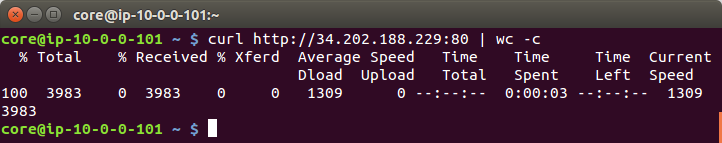
\includegraphics[width=0.6\textwidth]{images/figures/curl-wc.png}
\caption{Tamaño de la página principal solicitada en B.}
\end{figure}

El resultado es de 3983 B, que serán tomados como 4 kB a efectos de la estimación del coste.

Cada instancia que se ejecute dispone del uso de una dirección IP elástica gratuita. La presente infraestructura no necesita hacer uso de direcciones IP públicas adicionales por lo que la utilización de este recurso no supone un coste adicional.

En la Tabla \ref{tab:costepeticiones} se presenta el coste del tráfico externo anual proveniente de la transferencia de datos con direcciones IP elásticas para un determinado número de peticiones por hora, con un valor individual de 4 kB.

\FloatBarrier

\begin{table}
\begin{tabular}{ccc}
\hline
\rowcolor[HTML]{C0C0C0} 
\multicolumn{1}{|c|}{\cellcolor[HTML]{C0C0C0}\textbf{Peticiones/Hora}} & \multicolumn{1}{c|}{\cellcolor[HTML]{C0C0C0}\textbf{\begin{tabular}[c]{@{}c@{}}Transferencia de Datos/Hora\\ GB\end{tabular}}} & \multicolumn{1}{c|}{\cellcolor[HTML]{C0C0C0}\textbf{\begin{tabular}[c]{@{}c@{}}Coste anual\\ €\end{tabular}}} \\ \hline
\multicolumn{1}{|c|}{$1 * 10^6$}                                       & \multicolumn{1}{c|}{4}                                                                                                         & \multicolumn{1}{c|}{321,42}                                                                                   \\ \hline
\multicolumn{1}{|c|}{$2 * 10^6$}                                       & \multicolumn{1}{c|}{8}                                                                                                         & \multicolumn{1}{c|}{642,87}                                                                                   \\ \hline
\multicolumn{1}{|c|}{$4 * 10^6$}                                       & \multicolumn{1}{c|}{16}                                                                                                        & \multicolumn{1}{c|}{1.285,69}                                                                                 \\ \hline
\multicolumn{1}{|c|}{$8 * 10^6$}                                       & \multicolumn{1}{c|}{32}                                                                                                        & \multicolumn{1}{c|}{2.571,39}                                                                                 \\ \hline
\multicolumn{1}{|c|}{$16 * 10^6$}                                      & \multicolumn{1}{c|}{64}                                                                                                        & \multicolumn{1}{c|}{5.142,78}                                                                                 \\ \hline
\multicolumn{1}{|c|}{$32 * 10^6$}                                      & \multicolumn{1}{c|}{128}                                                                                                       & \multicolumn{1}{c|}{10.285,55}                                                                                \\ \hline
\multicolumn{1}{|c|}{$64 * 10^6$}                                      & \multicolumn{1}{c|}{256}                                                                                                       & \multicolumn{1}{c|}{22.628,31}                                                                                \\ \hline
\multicolumn{1}{|c|}{$128 * 10^6$}                                     & \multicolumn{1}{c|}{512}                                                                                                       & \multicolumn{1}{c|}{45.035,53} \\ \hline
\end{tabular}
\caption{Coste anual por instancia según el número de peticiones \label{tab:costepeticiones}}
\end{table}

En úlmimo lugar, existe la posibilidad de abaratar costes estableciendo una estrategia diferente a la del pago por uso. Entre ellas cabe destacar las siguientes:
\begin{itemize}
\item \textbf{Instancias de subasta}: Se puede pujar por capacidad informática libre en Amazon EC2 con descuentos de hasta el 90\% en comparación con el precio bajo demanda. Preferible para  aplicaciones solo viables con precios de computación muy bajos o para usuarios con necesidades de computación muy urgentes y voluminosas.
\item \textbf{Instancias reservadas}: Ofrece un descuento hasta del 75\% comparado con los precios de las instancias bajo demanda. Además, cuando se asignan instancias reservadas a una zona de disponibilidad específica, se proporciona una reserva de capacidad que se traduce en confianza adicional sobre la capacidad de lanzar instancias cuando se necesite. Son recomendadas cuando las aplicaciones tengan necesidades de estado constante o uso previsible y para usuarios que pueden comprometerse a utilizar Amazon EC2 durante un plazo de 1 o 3 años.
\item \textbf{Hosts dedicados}: Servidor físico de Amazon EC2 dedicado para su uso. Reduce costos permitiendo usar las licencias existentes de software enlazado al servidor. Se puede adquirir bajo demanda, por hora, o como reserva con un descuento de hasta el 70\% en comparación con el precio bajo demanda.
\end{itemize}

